% !TeX root = ../main.tex
% Add the above to each chapter to make compiling the PDF easier in some editors.

\chapter{Background and Related Work}\label{chap:background}

In this chapter we will look at some technologies and concepts 
that will be important for the understanding of the following chapters.
We will look at the QUIC protocol, which was our choice for the 
transport layer, eBPF, which we used for implementing the packet 
forwarding, Media over QUIC (MoQ), on top of which we built 
our example application and Adaptive Bitrate Streaming as well as 
Real-time Communication, which are fundamental concepts in the area 
of media streaming.
Finally, we will mention some related work, that tackles similar 
problems and provides interesting approaches.  

\section{QUIC}\label{sec:quic_bg}
% TODO: cite ~\parencite{quic-explained} for general explanation of QUIC
% TODO: cite \parencite{facebook-quic-usage} for QUIC usage at Facebook
% TODO: cite \parencite{google-quic-usage} for QUIC usage at Google
% TODO: cite \parencite{article-quic-usage} for general QUIC usage
Many fundamental internet protocols still used today have been around for 
a very long time.
For example, the Transmission Control Protocol (TCP) has been used as the backbone
of the internet for more than 40 years.
It has been designed to be reliable and to provide a connection-oriented
way of transmitting data, but the modern environment of the internet with
needs like lower latency, better multiplexing, or improved security makes it 
hard for TCP to keep up.
Limitations in the design and resulting issues like head-of-line blocking
have raised demand for a newly designed protocol that can keep up with the
modern internet. % TODO: head of line blocking citation
All of these issues, paired with the want for a more flexible development cycle
led to new creations.
QUIC, which started off as the ``Quick UDP Internet Connections'' protocol and has 
since been standardized by the IETF, with QUIC now being its own trademark, is a 
transport layer protocol built on top of UDP that is designed to be reliable, 
cryptographically secure and more performant than TCP\@.
QUIC, partly because it operates both in user- and kernel-space, has been designed to allow for a 
more rapid deployment cycle than TCP\@.
Similar to TCP, it is a connection-based protocol that uses TLS for encryption~\parencite{quic-explained}.
Back in 2018, QUIC was already the default protocol for the Google Chrome browser, which,
at the time, made up 60\% of the web browser market~\parencite{google-quic-usage}.
A little over two years later, Facebook, now Meta, was using QUIC for more than 75\% of 
their internet traffic which led to improvements regarding
request errors, tail latency, and header size~\parencite{facebook-quic-usage}.
As of August 2024, QUIC already made up 8.1\% of all internet traffic % TODO: update number
with support from pretty much every major browser
~\parencite{internet-quic-usage, article-quic-usage}.
On another note, Cloudflare-Radar has reportet, that at point of writing this thesis, 
30\% of HTTP traffic is HTTP/3, which uses QUIC~\parencite{cloudflare-radar}.
With big players like Google, Meta, or Microsoft putting emphasis on
using QUIC to improve their services, this number will likely increase even further.

\subsection{Connections and Streams}
Since QUIC is a connection-based protocol, some initial overhead to establish a connection is needed.
However, the design incorporates features that aim for an efficient way of establishing 
connections, e.g.\ by using 0-RTT (zero round-trip-time) handshakes. 
Latency improvements like the 0-RTT handshake, however, come at the cost of security since that opens 
the door for replay attacks.
QUIC's 1-RTT handshake does not have this issue, while still being faster
than e.g.\ the handshake of TCP/TLS, since it handles all setup tasks using only
a single round trip.
Another part where QUIC tries to optimize connection management is the use of streams.
Streams are designed to be lightweight and can be opened without the need for a handshake.
This goes as far as one single packet being able to open a new stream, transferring stream data,
as well as closing the stream again.
This allows for new techniques to improve data transmission and will also be part of the fast-relay 
setup in this thesis.
Aside from streams it is also possible to send data via unreliable 
datagrams~\parencite{rfc-9221}.
This is possible since QUIC is based on UDP\@.
It further improves the versatility of the protocol and allows 
for new ways of optimizing data transmission.

\subsection{quic-go}
There are many implementations of the QUIC protocol available, providing libraries for a lot of 
today's most popular programming languages.
The implementation we settled on for this thesis is the quic-go library which provides a pure Go 
approach to implementing the standards of RFC-9000~\parencite{rfc-9000}, 
RFC-9221~\parencite{rfc-9221} as well as some others which are not 
important for our usecase. 
However, since we need some special behavior of the userspace part of QUIC, we will introduce some 
modifications into quic-go.  
Those modifications will be explained further in~\autoref{sec:quic_adaptions}.

\subsection{QUIC's Importance to Fast-Relays}
The QUIC protocol will be a fundamental part of the fast-relay setup in this thesis, yet the ideas used 
to make relays faster is not limited to QUIC\@.
QUIC is chosen as an example protocol due to its increasing popularity, which offers big potential 
in early adoption and deployment of fast-relays.
Also, the easy incorporation of changes into libraries providing RFC implementations makes it a good 
starting point for experimenting with what can and cannot be done regarding our research questions.
This includes the possibility of neglecting the difficulties that the heavy encryption of QUIC brings with 
it by just turning off the related functionality.
Another reason we opted for QUIC is that it allows for easy packet dropping.
In order to do that we just need to send each frame in a lightweight unidirectional stream and in 
case of a drop of said frame, we can just close the corresponding stream.
This would not be possible with TCP, due to its reliability-based nature.

% This includes the possibility of mitigating missing technologies, mainly for offloading QUIC % TODO: better wording?
% decryption and encryption onto hardware.
% To conquer that, the existing protocol libraries can be modified easily to simulate any needed behavior.
\section{eBPF}\label{sec:ebpf_bg}
In 1992 a technology called ``Berkeley Packet Filter'' (BPF) was introduced into 
the Unix kernel.
By using BPF, it is possible to attach a small BPF program to some pre-defined hook points in 
the network stack of the kernel and filter packets there in a stateless manner.
This provided more efficiency since the packets did not need to be copied into 
userspace anymore but could be processed directly in the kernel.
A need for better tracing capabilities of the Linux kernel then led to the development 
of an extended version of BPF called ``eBPF'' which was introduced in 2014 and 
heavily influenced by a tracing tool called ``dtrace'', which allows for 
real-time inspection of running processes, memory- and CPU-usages, network-resources 
and more~\parencite{ebpf-intro-tigera}.

\subsection{eBPF Hook Points}
The Linux kernel offers several hook points to which eBPF programs can be attached.
There are two prominent ones that we considered for our suggested setup.
The first allows access to the Traffic Control (TC) subsystem, while the 
second allows access to the eXpress Data Path (XDP) subsystem.

XDP would generally provide a better performance since it is located 
lower on the network stack, namely directly in the NIC driver, than the 
TC-hook point, which is located in the link layer.
On the other hand, TC offers a more versatile way of packet processing since 
the used \verb|sk_buff| buffer object containing the packet data provides access to metadata, which is unavailable when using XDP and its \verb|xdp_buff| buffer object.
% https://liuhangbin.netlify.app/post/ebpf-and-xdp/ % TODO: is this citable?
What ultimately led us to choose TC over XDP was, however, the fact that 
XDP only allows ingress packet processing, while TC allows processing packets at ingress and egress.
That means that with XDP, we would not have been able to redirect packets to be handled 
at egress, which is crucial for the fast-relay setup we aim for. % TODO: cannot redirect from XDP to TC?

% The XDP hook, which is directly located in the NIC-driver, lies lower in the network 
% stack than the TC-hook, which is located in the link-layer.
% Despite being higher up in the network stack, the TC-hook has the big advantage that
% it offers ingress and egress processing while the XDP-hook is available for ingress 
% processing only.
% This makes the XDP-hook suboptimal for implementing fast-relays since 
% they heavily rely on processing packets at egress after those were redirected
% from ingress.
\autoref{fig:ebpf-hooks} illustrates again the relative positions of the TC and
XDP hook points in the network stack.

\begin{figure}[H]
    \centering
    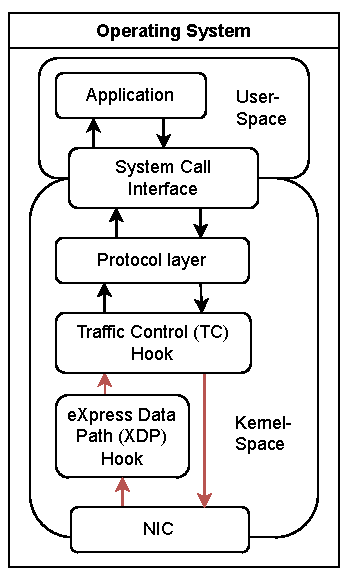
\includegraphics[width=0.3\textwidth]{figures/02_background/hook-point-locations.drawio.pdf}
    \caption[Hook points within network stack]{TC and XDP hook points in the Linux kernel.
    The red loop indicates the ``short-cut'' that the fast-relay utilizes.
    }\label{fig:ebpf-hooks}
\end{figure}

% \subsection{Traffic Control Queuing Disciplines} % TODO: needed?
% The Linux Traffic Control Subsystem uses Queuing Disciplines (qdiscs) to define how packets
% are handled. TODO

\subsection{eBPF Verifier}
Since eBPF programs are executed in the kernel, it is quite obvious that extensive
security checks need to be in place to ensure that the kernel does not experience 
problems like infinite loops, accesses to invalid memory locations, or other security 
related issues.
This explains the existence of the so-called ``eBPF verifier'' which inspects 
every eBPF program for its safety by simulating possible program paths, 
looking at the graph representation of the program and more~\parencite{ebpf-verifier}.
This imposes some restrictions on the complexity of the programs that can be 
used within the kernel.
For our early prototype implementation, this does not cause any issues, since we do not need 
to rely on very complex control structures.
However, if one wants to extend the prototype to support a more complicated packet structure
(e.g.~composition of multiple frames per packet), the verifier might become a limiting factor.


\subsection{Important eBPF Concepts}
One of the most important concepts in eBPF, which we use quite extensively, is 
the ``eBPF-map''.
Such a map boils down to a section in memory that is reserved for the eBPF program
and which can be used as a key-value store for arbitrary data.
This part of memory can then also be accessed from userspace and thus provides the main 
way of communication between the eBPF program and our application.


\vspace{0.5cm}
\noindent\begin{minipage}{\textwidth}
    \begin{lstlisting}[style=CStyle,caption={Examplary eBPF map definitions.}, label={lst:ebpf-map}]
        struct {
            __uint(type, BPF_MAP_TYPE_HASH);        // Hash map
            __type(key, struct client_info_key_t);  // Specific client key
            __type(value, uint32_t);                // 32 bit id
            __uint(max_entries, MAX_CLIENTS);       // Maximum number of clients
            __uint(pinning, LIBBPF_PIN_BY_NAME);    // Pin by name to the tc filesystem
        } client_id SEC(".maps");

        struct {
            __uint(type, BPF_MAP_TYPE_RINGBUF);     // Ring buffer
            __uint(max_entries, MAX_PACKET_EVENTS); // Maximum number of packet events
            __uint(pinning, LIBBPF_PIN_BY_NAME);    // Pin by name to the tc filesystem
        } packet_events SEC(".maps");
    \end{lstlisting}
\end{minipage}
\vspace{0.5cm}

When we define an eBPF-map, we can choose between different types and configure
size, key type, value type, and how the map is stored. % TODO: surely there is more one can define
An example of two eBPF-map definitions can be seen in~\autoref{lst:ebpf-map}.
It shows two different types of maps, a hash map, and a ring buffer, that are used in
our fast-relay setup.
Those and other relevant map types are listed in~\autoref{tab:ebpf-map-types}.


\vspace{0.5cm}

\begin{table}[H]
    \centering
    \begin{tabular}{L{7cm}L{7cm}}
        \toprule
            Type & Description \\
        \midrule
            BPF\_MAP\_TYPE\_HASH & A hash map where keys and values can be arbitrarily defined. \\
        \midrule
            BPF\_MAP\_TYPE\_PERCPU\_HASH & A hash map with separate value slots for each CPU, providing improved performance in multi-core environments. \\
        \midrule
            BPF\_MAP\_TYPE\_ARRAY & An array map that allows random access to elements by index. \\
        \midrule
            BPF\_MAP\_TYPE\_PERCPU\_ARRAY & An array map with separate value slots for each CPU, useful for per-CPU data storage. \\
        \midrule
            BPF\_MAP\_TYPE\_RINGBUF & A ring buffer for implementing high-performance data queues. \\
        \bottomrule
    \end{tabular}
    \caption[Subset of eBPF map types]{Some eBPF map types. (defined in /usr/include/linux/bpf.h)}\label{tab:ebpf-map-types}
\end{table}


\section{Media over QUIC (MoQ)}\label{sec:moq_bg}

\iffalse % TODO: remove (only notes)

Notes on: https://www.ietf.org/blog/moq-overview/

Target: live streaming, real-time collaboration, gaming, etc.

Good scaling capabilities cause high latency
Low latency systems have poor scaling capabilities

MoQ aims for low latency and high scalability
Built on top of raw QUIC (or WebTransport)

Maybe add quote from https://datatracker.ietf.org/wg/moq/about/

Publisher / Subscriber model
Support for many formats, rate adaptation, cache friendly mechanisms, etc.
Relays function as caches for lower latency and higher quality

Took approaches from RTP (real-time stuff), HLS/DASH (scaling)

If many downstream requests for same data, relay only needs one copy

Media content can be end-to-end encrypted but relay can still access metadata
like priority field - this is similar to our setup.
% TODO: how can these fields still be accessed? are they just not encrypted?
Priority can be used when caching or when forwarding under congestion.
The MoQ can drop or delay certain media if necessary.

VoD consumption >> live streaming but live makes up most of peak traffic

MoQ will have great influence on real-time collaboration infrastructure like 
Zoom, Teams, etc.~and live streaming platforms like Twitch, YouTube, etc. 

low latency, high fan out, high scalability is pretty much ideal for most apps.

(Also psychological improvement since latency problems tend to be blamed on the 
other party, not the network.) % TODO: prolly no fit in this section?
https://blog.webex.com/hybrid-work/how-latency-harms-collaboration/

\fi

% \subsection{What is Media over QUIC (MoQ)?} % TODO: maybe not needed
On the application layer we will use the Media over QUIC (MoQ) protocol which 
is as of summer 2024 still being in the process of standardization by the IETF\@.
MoQ targets live-streaming and real-time collaboration applications like Zoom,
Microsoft Teams, or Google Meet.
It is built on top of the QUIC protocol with the possibility of using WebTransport
for browser support.
A general publisher/subscriber model is used and the draft tries to combine
performant approaches from protocols like RTP (for real-time features) and HLS/DASH
(for scalability).

\subsection{Solving Scaling versus Latency}
For a long time now there have been two different camps with regards to media-data-
transmission-protocols and -setups.
One is heavily focused on low latency while the other is aiming for high scalability.
Systems of the former kind include real-time collaboration tools like aforementioned
Zoom, Teams, or Meet.
The latter ones are often huge platforms like Twitch, YouTube or Netflix which need to 
reach millions of users at the same time.
The one thing both have in common is that it turns out to be difficult to incorporate both 
low latency and high scalability into the system at the same time.
The MoQ protocol tries to solve this by providing a setup that is both low-latency and
highly scalable.
To achieve this it supports performance enhancing approaches like relay caching or support 
for adaptive rate mechanisms. % TODO: other things that are used to achieve this?

\subsection{Design of a MoQ Relay}
The charter for the IETF working group describes what MoQ, and therefore also a relay 
that wants to meet the MoQ requirements, needs to support.
These requirements for the publication- and distribution-setup mention the support of 
multiple formats, dynamic rate adaption mechanisms (e.g.~used for congestion handling)
as well as cache-friendly mechanisms.

\begin{figure}
    \centering
    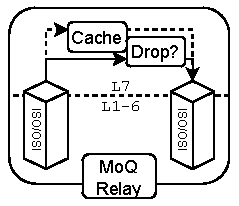
\includegraphics[width=0.3\textwidth]{figures/02_background/moq-relay.drawio.pdf}
    \caption[Rough MoQ relay architecture]{Rough MoQ relay architecture.}\label{fig:moq_relay_architecture}
\end{figure}

Figure~\ref{fig:moq_relay_architecture} gives a visualization of the rough architecture
of a MoQ relay.
It hints at key components like the relay level cache and the congestion handling
mechanism.
What one can also infer is the place of MoQ in the OSI-model namely at the application
layer which itself builds on top of lower level protocols like QUIC, UDP, IP and Ethernet.
In figure~\ref{fig:non_caching_relay_data_request} and figure~\ref{fig:moq_relay_data_request} 
one can see a comparison between the delayed fan-out of the media content caused by the MoQ 
relay and a more traditional setup.
The former is able to reduce the traffic through a network by making multiple transmissions
of the same data between server and relay obsolete.

\begin{figure}[!htb]
    \begin{minipage}{0.45\textwidth}
        \centering
        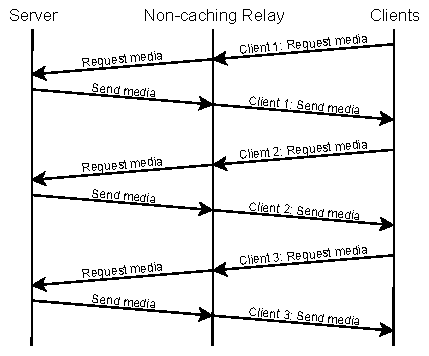
\includegraphics[width=1\linewidth]{figures/02_background/non-caching-relay-data-request.drawio.pdf}
        \caption[Non-caching relay traffic]{Multiple data transmissions for different clients.}\label{fig:non_caching_relay_data_request}
    \end{minipage}\hfill
    \begin{minipage}{0.45\textwidth}
        \centering
        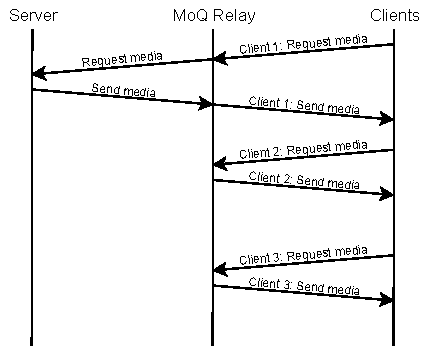
\includegraphics[width=1\linewidth]{figures/02_background/moq-relay-data-request.drawio.pdf}
        \caption[MoQ relay traffic]{Only single data transmission towards the relay.}\label{fig:moq_relay_data_request}
    \end{minipage}
\end{figure}

This caching mechanism fits quite naturally into our proposed eBPF setup since we will need to 
communicate packet data between kernel- and user-space anyway to keep the QUIC library in a 
consistent state.
In addition to that the congestion handling functionality of the MoQ relay can also
be integrated fairly easy within eBPF\@.
This is because packet dropping is ultimately one of the main use cases of plain eBPF 
programs and as such easy to implement.
In a later section will go into detail on how the eBPF setup actually uses mechanisms like 
priority fields for this and how those meet the standard specifications.

\subsection{moqtransport}
In order to use the MoQ protocol in our setup we will make use of a library that implements 
the MoQ transport protocol (moqtransport or MoQT) in Go~\parencite{priority-moqtransport-repo}
The goal of MoQT is to define a media transport protocol that is operating on top
of QUIC and WebTransport which is providing the concrete designs that the charter of 
the MoQ working group is aiming for.
This includes, for example, actual structure of the different message types or error handling in case 
of a wrong state.
As of writing this thesis the MoQT draft is in its fifth version~\parencite{draft-moqtransport}.

% Besides that the fast-relay implementation will also make use of the moqtransport library.
% This library brings the `Media over QUIC' (MoQ) protocol to Go and will be used as a media transport protocol 
% when looking at the impact of fast-relays on adaptive real-time video streaming.
% The MoQ protocol is being standardized by the IETF since July 2023 and has yet to be finalized. 
\section{Real Time Communication and Adaptive Bitrate Streaming}\label{sec:rt_and_adaptive_bitrate_streaming}

Whenever we look at different types of streaming it is important to consider the 
different requirements that come with them.
We differentiate between a one sided communication, where an increase in delay 
in order to gain a higher quality is acceptable, and a two sided communication, 
where a low delay is crucial for satisfactory user experience.
The former allows for more complex setups like the one considered in subsection
\nobreakspace\ref{subsec:adaptive_bitrate_streaming} while the latter requires
a more direct approach which will be discussed in the following subsection.

\subsection{Real Time Communication}
When looking at streaming setups that consider real-time constraints, such as conferencing 
where interhuman communication is involved, the objectives of the connection tend towards
low latency.
In order to provide natural feeling human communication, the delay between the sender 
and the receiver has to be minimal.
This type of communication between devices is often referred to as ``Real-Time Communication'' 
(RTC) and used in many applications, such as Zoom, Skype, or Discord.

\subsubsection{Mechanisms and Ideas}
The main goal of such systems is to minimize the delay between the sender and the receiver
while additionally allowing all parties to communicate with each other.
A lot of design decisions are made with this in mind.
One design decision for a large conferencing system like Zoom
might consider the usage of peer-to-peer (P2P) connections versus a server-based
approach.
While P2P might allow for lower latencies in case of a small number of participants,
a server-based approach scales a lot better and can therefore provide a better
ressource utilization.

\subsubsection{Implications on Streaming Setup}
The need for low latency also has implications of the specific setup at hand.
An example of such an implication is the design of the connection between the 
real-time connection network (RTCN) and a client.
Since retransmissions are expensive in terms of latency, a setup should strive to minimize 
the distance a packet has to travel through an unreliable network.
This could be achived by having multiple, strategically placed, eddge-servers, which internally use 
a, compared to the internet, more reliable connection, for longer (e.g.~intercontinental) connections.
This way packet loss occuring during the client-to-edge-server connection would not have a big 
impact on the overall latency of the connection.
A visualization of such an appraoch can be seen in~\autoref{fig:real-time-streaming-connections}.

\vspace{0.5cm}
\begin{figure}[H]
    \centering
    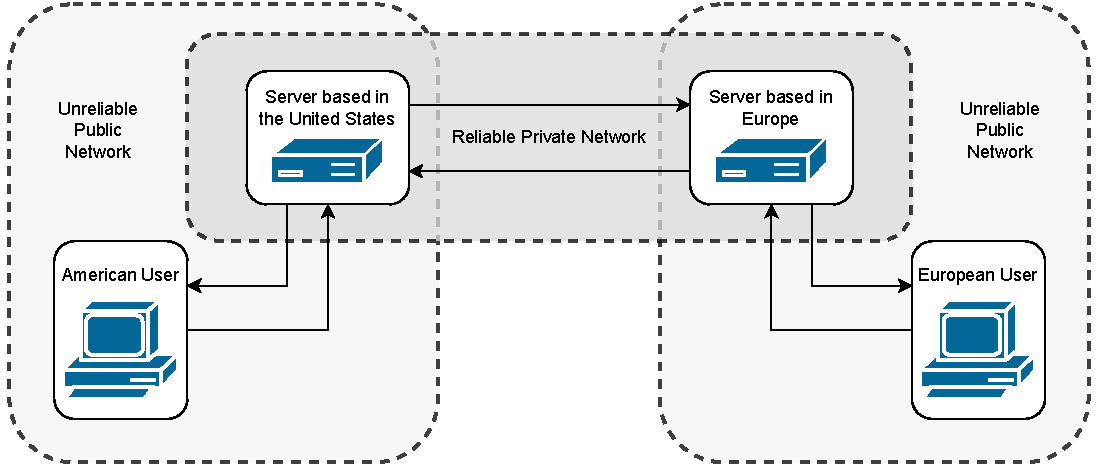
\includegraphics[width=0.8\textwidth]{figures/02_background/real-time-streaming-connections.drawio.pdf}
    \caption[Real-time streaming connections]{A setup with multiple edge-servers around the world
    can help to minimize the latency of a connection.}\label{fig:real-time-streaming-connections}
\end{figure}

\subsection{Adaptive Bitrate Streaming}\label{subsec:adaptive_bitrate_streaming}
Multimedia streaming is a big part of the internet and many optimizations have
been developed to improve the quality of service for the end-users.
This includes considering (in real-time) parts of the clients' connection state, 
such as available bandwidth, and adapting the rate at which a server sends data.
Such a process is called ``Adaptive Bitrate Streaming'' (ABS) and is employed in many 
of today's streaming setups.

% TODO: cite    https://netflixtechblog.com/optimizing-the-netflix-streaming-experience-with-data-science-725f04c3e834
% TODO:         https://www.cloudflare.com/de-de/learning/video/what-is-adaptive-bitrate-streaming/
% TODO:         https://docs.imagekit.io/features/video-transformation/adaptive-bitrate-streaming
\vspace{0.5cm}
\begin{figure}[H]
    \centering
    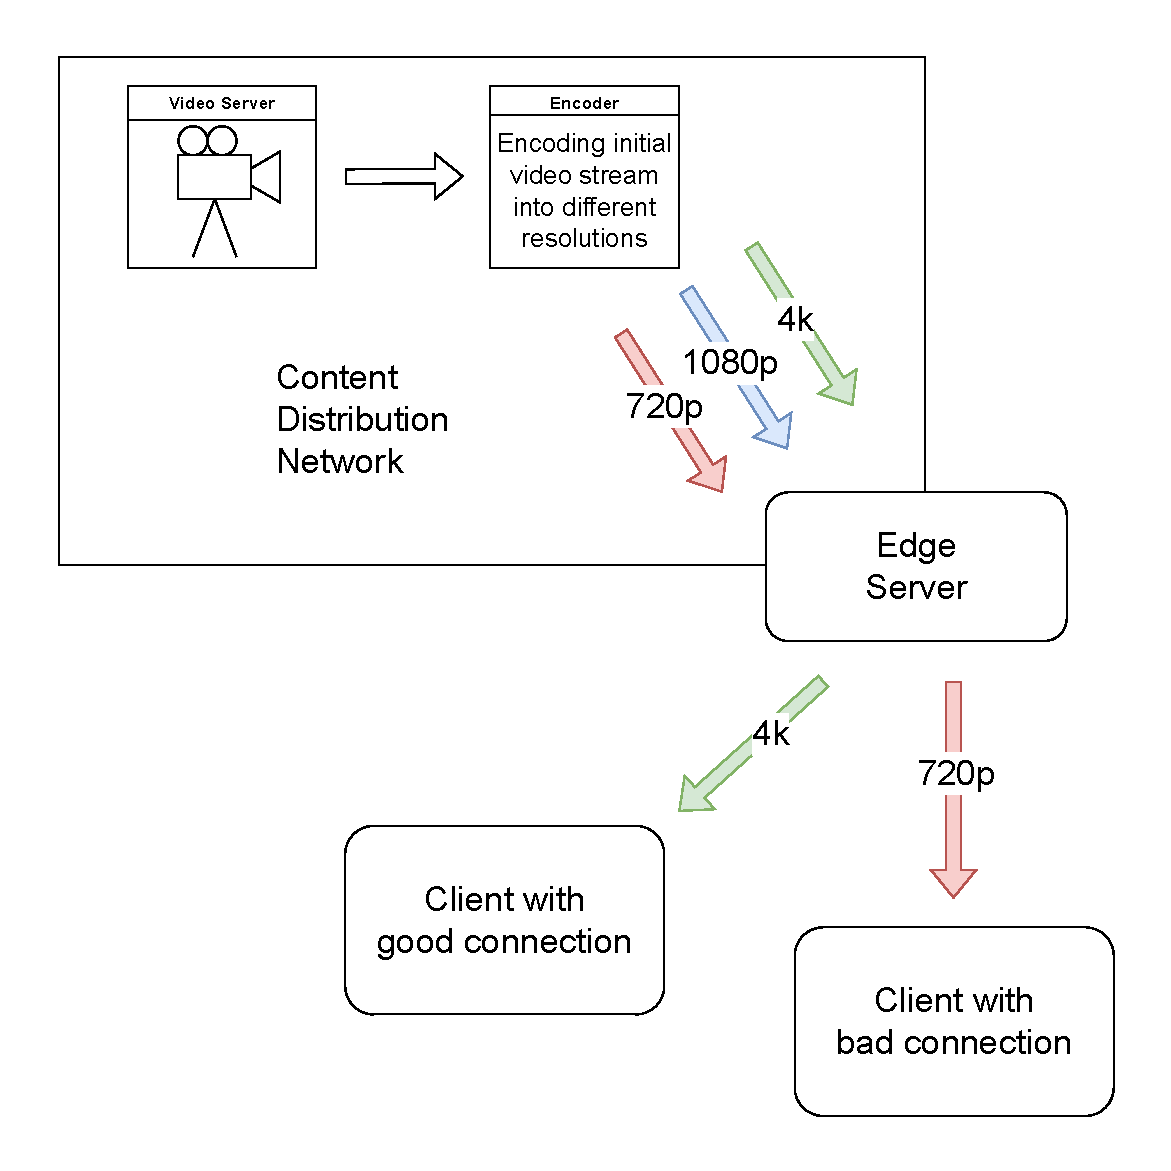
\includegraphics[width=\textwidth]{figures/02_background/adaptive-bitrate-streaming.drawio.pdf}
    \caption[Adaptive streaming schematic]{Behind the scenes multiple streams with different
    resolutions exist to allow adapting to a user's bitrate.}\label{fig:adaptive-bitrate-streaming}
\end{figure}
% The way the example implementation of fast-realys in this thesis is set up,
% is that the video server will encode into each packet its priority.
% For example I-frames have a high priority while P-frames have a lower
% priority.
% The relay then can decide not to forward certain packets to a client if
% the client is experiencing congestion.
\vspace{1cm}

\subsubsection{Mechanisms and Ideas}
ABS implements the simple idea of changing the amount of data sent to a client 
based on the clients' connection quality.
This means a client with a good connection gets a higher-quality stream than 
one with a bad connection.
For this, the internal setup needs to be able to provide multiple streams with
different resolutions and bitrates.
An example setup can be seen in~\autoref{fig:adaptive-bitrate-streaming} where
an encoder creates streams with different resolutions and an edge server, that 
manages the connections to the clients, can switch between those streams based on
the connection state of a specific client.
Twitch and YouTube-Live are examples where, although more complex, similar setups
are used to provide a better user experience.
The premise of such a setup is that in case of a bad connection, it is still 
preferable to be able to watch a stream continuously, even if that means
cutting down on quality.
When looking at such real world examples, however, it is important that one keeps 
the differences between Video-on-Demand (VoD) and live-streaming in mind.
The latter might require more computation before a video is sent since the media 
has to be processed on the fly since it is created in real-time.
For VoD on the other hand the media already exists in its final form. 

\subsubsection{Implications on Streaming Setup}
ABS forces a few changes to the way servers and relays are set up.
First, as figure~\autoref{fig:adaptive-bitrate-streaming} shows, there needs to 
be an ``encoding'' component that turns the single, high-quality stream that is 
received from the streaming source into multiple streams with different resolutions.
Besides that, the relay needs to keep track of the clients' connection quality, e.g.~using 
measurements like RTT, packet loss, etc., and decide which stream to forward to the client.
Since the connection quality can change dynamically the relay also needs to continuously
monitor each connection and potentially change the used stream.
Besides encoding and monitoring aspects the system also has increased storage requirements
since stream data will essentially be duplicated.

\section{Related Work}\label{sec:related_work}

Our approach combines ideas from multiple different 
related publications.
This section will give a brief overview of some related work 
that uses similar concepts such as packet handling using a BPF 
program or bypassing the Linux network stack to improve performance.

\subsection{eQUIC Gateway}
There have been previous publications on making QUIC more efficient by using BPF programs
such as~\parencite{equic-gateway}, where a BPF program is used together with the Linux
eXpress Data Path (XDP) to filter packets based on information provided by the userspace.
This approach provided significant performance improvements with an increase of throughput
by almost a third and a reduction of CPU time consumption caused by filtering packets by
more than 25\%.
This shows that a setup leveraging Linux kernel features such as BPF has a lot of potential
to improve the current infrastructure.
% TODO: more specific info on how this paper's setup looks like / differs from ours?
% TODO: mention that XDP is not feasible for our setup because it has no egress hook?

\subsection{Kernel Bypass}
Another interesting approach that follows a similar idea of speeding up packet processing
by avoiding the Linux network stack is~\parencite{kernel-bypass-msc-thesis}.
The difference in this work is that DPDK is used to bypass the network stack to 
then process packets in userspace instead of directly using eBPF programs for processing,
as we do.
This, for example, offers more flexibility as the userspace program is not as limited (e.g.\ 
by the eBPF verifier) as the eBPF program but might also lead to slightly more system calls,
especially in the setup of a system, when user- and kernel-space need to communicate, thus 
increasing latency.
% TODO: clear enough / everything covered and correct?

\subsection{Priority drop}
The idea of dropping packets based on their priority to adapt a connection
in a congestion event has also been around for a while.
This is explored further in~\parencite{media-streaming-prio-drop}.
There the authors discuss a more tailorable congestion handling 
compared to video quality discretization as well as an improvement 
to, potentially randomized, frame dropping.
This thesis, similar to~\parencite{media-streaming-prio-drop}, will not focus
on how the priority for a specific packet is determined but rather on how
packets are handled in general.
For this, it is assumed that a higher-level protocol has correctly determined 
the packet priorities and can handle the drop of packets with lower priority
in case of limited bandwidth.
% TODO: explain more on different ways of encoding priorities e.g. I- and 
% TODO: P-frames in video streaming?
\section{Summary}\label{sec:summary_ch2}

In this chapter we have introduced some prerequisites for the 
upcoming one.
We have looked at the QUIC transport protocol and the MoQ protocol, which is 
based on top of QUIC\@.
We have also mentioned eBPF and presented two different concepts in the 
realm of streaming, namely ABS and RTC\@.
In the next chapter, we will combine these concepts to create a 
relay design that is capable of traffic forwarding.
We will do so by first mentioning necessary changes to the library 
implementing the QUIC standard, then we will explain our proposed eBPF setup 
and finally, we will go into detail on special considerations like 
userspace synchronization or congestion related topics.